\par
In this chapter, I report the summer 2023 internship work at LBNL and additional numerical implementations I continued to finish this thesis.

As we mentioned in Chapter \ref{sec:intro_complex_fluid}, we consider the deviatoric stress tensor of the form as in equation (\ref{eq_CN_tau}), 
\begin{equation}
  \boldsymbol{\tau} =
  \nu_0  \bm{A}_1 +  \nu_1  \bm{A}_1^2 + \nu_2 \bm{A}_2 ,
\nonumber
\end{equation}
where each $\nu_i$ for $i = 0,1,2$ is dependent on the materials or flow types. In this project, we explore two examples: 1) granular materials and 2) non-colloidal suspension in a Newtonian fluid. While the big picture of a viscous term is the same as described in equation (\ref{eq_CN_tau}), the way to obtain the coefficients $\nu_i$ are different. We thus address establishing the viscosity terms first for both examples. Then, we examine each flow in geometry by solving the Navier-Stokes equation,
in which they were introduced in Chapter 1; equations (\ref{eq_conserv_mass}) and (\ref{eq_momentum_NS}).
\par
In the AMReX-incflo code, we can only use the explicit Euler time integration method due to the stress tensor $\bm{\tau}$ having a quadratic relationship with the strain rate $\bm{D}$, which is a function of the velocity $\vec{u}$. 
To clarify, we write the tensor $\bm{\tau}$ in terms of $\bm{D}$ explicitly,
\begin{equation}
  \boldsymbol{\tau} =
  2 \nu_0  \bm{D} +  2 \nu_1  \bm{D}^2 
  + 2\nu_2 \left(
    \frac{\partial \bm{D}}{\partial t} + 
     \vec{u} \cdot \nabla \bm{D}
    +\bm{D} \nabla \vec{u}+ \left(\nabla \vec{u} \right)^T \bm{D} 
   \right)
\end{equation}
% Let's look at the last term a little more closely:
% \begin{equation}
%   \nu_2 \left(
%    \frac{\partial }{\partial t}\left( \nabla \vec{u} +  \nabla\vec{u}^T \right) + 
%     \vec{u} \cdot \nabla \left(  \nabla\vec{u} +  \nabla\vec{u}^T \right) 
%    +\left(  \nabla\vec{u} + \nabla \vec{u}^T \right)  \nabla \vec{u}+ \left(\nabla \vec{u} \right)^T \left(  \nabla\vec{u} +  \nabla\vec{u}^T \right) 
%   \right)
% \end{equation}
% \begin{equation}
%   \nu_2 \left(
%    2\frac{\partial \bm{D} }{\partial t}
%    + \left(\nabla\vec{u}  \right)^2
%   + 2(\nabla \vec{u})^T  \nabla \vec{u}+
%    \left(    \nabla\vec{u}^T \right)^2
%   \right)
% \end{equation}
To achieve second-order convergence, we implement two more time integration methods in AMReX-incflo. As a simpler step, we coded the explicit Runge-Kutta 2 (RK2) scheme. We then attempt to use a predictor-corrector method, which is a fully implicit formula.
\par
The order of this chapter is the following. We explain the computation of viscosities for granular materials and non-colloidal suspension in a Newtonian fluid. Then, we discuss the numerical methods,   Then,  We close this chapter by showing some numerical results.

\section{Granular rheology}
Depending on the level of stress, viscoplastic fluids either flow or act like rigid solids. The minimum value that makes viscoplastic fluids move is called yield stress. 
We can easily find viscoplastic materials in our lives; for example, toothpaste, and whipped cream. 
Among many different types, we particularly study those granular materials. They are also considered viscoplastic fluids, depending on the states. For instance, a medicine tablet (pill) is considered a solid. However, the powder of ingredients acts as a fluid since it flows. 
There are many factors we need to learn to have a full understanding of granular materials' behavior.
Since the yield stress is the main value to understand different phases (liquid vs solid) of continuum granular flow, we focus on computing more accurate stress, by taking pressure into account. The source of pressure can be friction between granular matters or external forces.  
We consider both the shear stress rate and the pressure onto the granular materials as the sources of yield stress. 
\par
In Chapter 1, we introduced the stress tensor for the fluid momentum equation in equation (\ref{eq_stress_tensor}). 
We now express a new stress tensor $\bm \tau$ with a higher-order strain rate that can describe non-isotropic (meaning material properties changes along with direction) flow effects,
\begin{align}
  \bar{\bar{\sigma}}
    = -P \bar{\bar{I}}  + \bm{\tau}
    =  -P \bar{\bar{I}}  
    + \mu_1(\dot{\gamma}) \mathcal{O}({\bm D})
    + \mu_2(\dot{\gamma}) \mathcal{O}({\bm D^2}).
  \end{align}
In this section, we focus on the methodology to compute the viscosity $\mu_i ({\dot{\gamma}})$ ($i = 1,2$) under the simple shear flow. 
% A new apparent viscosity computation using the well-known $\mu(I)$ relation can also be found [{\color{blue}REFERENCE}]. 


To describe a non-isotropic flow, we consider the deviatoric stress tensor of the form (\ref{eq_2ndOrder_tau}), which is derived under two conditions:
(1) the flow motion is simple with a constant stretch history by neglecting deformation history, and (2) the flow is isochoric, having uniform properties along streamlines and tr$(D) = 0$. 
In particular, we see \cite{srivastava_viscometric_2021}
% \begin{align*}
% \bar{\bar{\sigma}} - P {\bm I} \equiv
%   {\bm {\bm \tau}}
%   =  \ \mu_1 {\bm D} 
%   + \mu_2  \left[ {\bm D}^2  - \frac{\text{tr}\left({\bm D}^2\right)}{3}{\bm I} \right]
%   + \eta_3  \left[ {\bm D}{\bm W} - {\bm W}{\bm D} \right]
%   \nonumber \\
%   + \frac{\kappa_1}{\dot{\gamma }^2} \bm D 
%   + \frac{\kappa_2}{\dot{\gamma }^2}  \left[ {\bm D}^2  
%   - \frac{\text{tr}\left({\bm D}^2\right)}{3}{\bm I} \right],
% \end{align*}
\begin{equation}
  {\bm {\bm \tau}}
  = \mu_1(\dot{\gamma}) {\bm D}
  \ +  \ 
 \mu_2 (\dot{\gamma})
  \left[ {\bm D}^2  - \frac{\text{tr}\left({\bm D}^2\right)}{3}{\bm I} \right],
  % \ + \
  % \left( \mu_3 \dot{\gamma}^2 \right)
  % \frac{1}{\dot{\gamma}^2}
  %   \left[ {\bm D}{\bm W} - {\bm W}{\bm D} \right]
\label{eq_2ndOrder_tau}
\end{equation}
where 
\begin{equation}
  \mu_1 (\dot{\gamma})
   = \left( \eta_1 \dot{\gamma}+ \kappa_1 \right) \frac{1}{\dot{\gamma}},
\label{eq_mu1_main}
\end{equation}
and 
\begin{equation}
  \mu_2 (\dot{\gamma}) = 
  \left( \eta_2  \dot{\gamma}^2
  +  \kappa_2 
  \right) \frac{1}{\dot{\gamma}^2}
  \label{eq_mu2_main}
\end{equation}
Note that the magnitude of strain rate, $\dot{\gamma}$, can be computed by applying the scaled Frobenius norm for a second-order tensor, 
\[
  \dot{\gamma}  = |\bm{D}| = \sqrt{\frac{1}{2}
    \text{tr}\left(\bm{D} \bm{D}^{T} \right)}.
\]
In general, the Frobenius norm states $\bm{D}^H$ instead of $\bm{D}^T$. Since we consider real-valued tensors, it is valid to have $\bm{D}^H = \bm{D}^T$.
\par
We also note that the functions, $\eta_i$ and $\kappa_i$ for $i = 1,2$, have the following dependency to the total stress: each $\eta_i(\dot{\gamma}, p)$ is (shear) rate-dependent and $\kappa_i (p)$ is (shear) rate-independent. 
Along with the shear effect from $\eta_1$, we can observe the second normal-stress difference in shear flows from $\eta_2$.
The rate-independent terms, $\kappa_1$ and $\kappa_2$, allow us to find yield stress. 
We explain the details of these two types of functions in the following sub-section.

\subsection{$\mu (I)$ rheology}
The main key to getting $\eta_i$ and $\kappa_i$ terms is the well-known $\mu(I)$ relationship developed by \textit{Jop, 2006}~\cite{jop_constitutive_2006}.
Here, $I$ is called the \textit{inertial number} defined as 
\begin{equation}
  I =  \frac{\dot{\gamma} d }{\sqrt{P/\rho_p}},
  \label{eq_inertialI}
\end{equation}
where $d$ and $\rho_p$ are the average particle diameter and density of given granular material.
This dimensionless quantity describes the average static force compared to the inertial force between granular particles. Jop, in~\cite{jop_constitutive_2006}, interpreted the inertial number as the ratio between a macroscopic deformation and an inertial timescale. 
\par
We bring an hourglass example to describe the granular flow regimes depending on the inertial number. 
\begin{figure}[ht]
  \begin{center}
    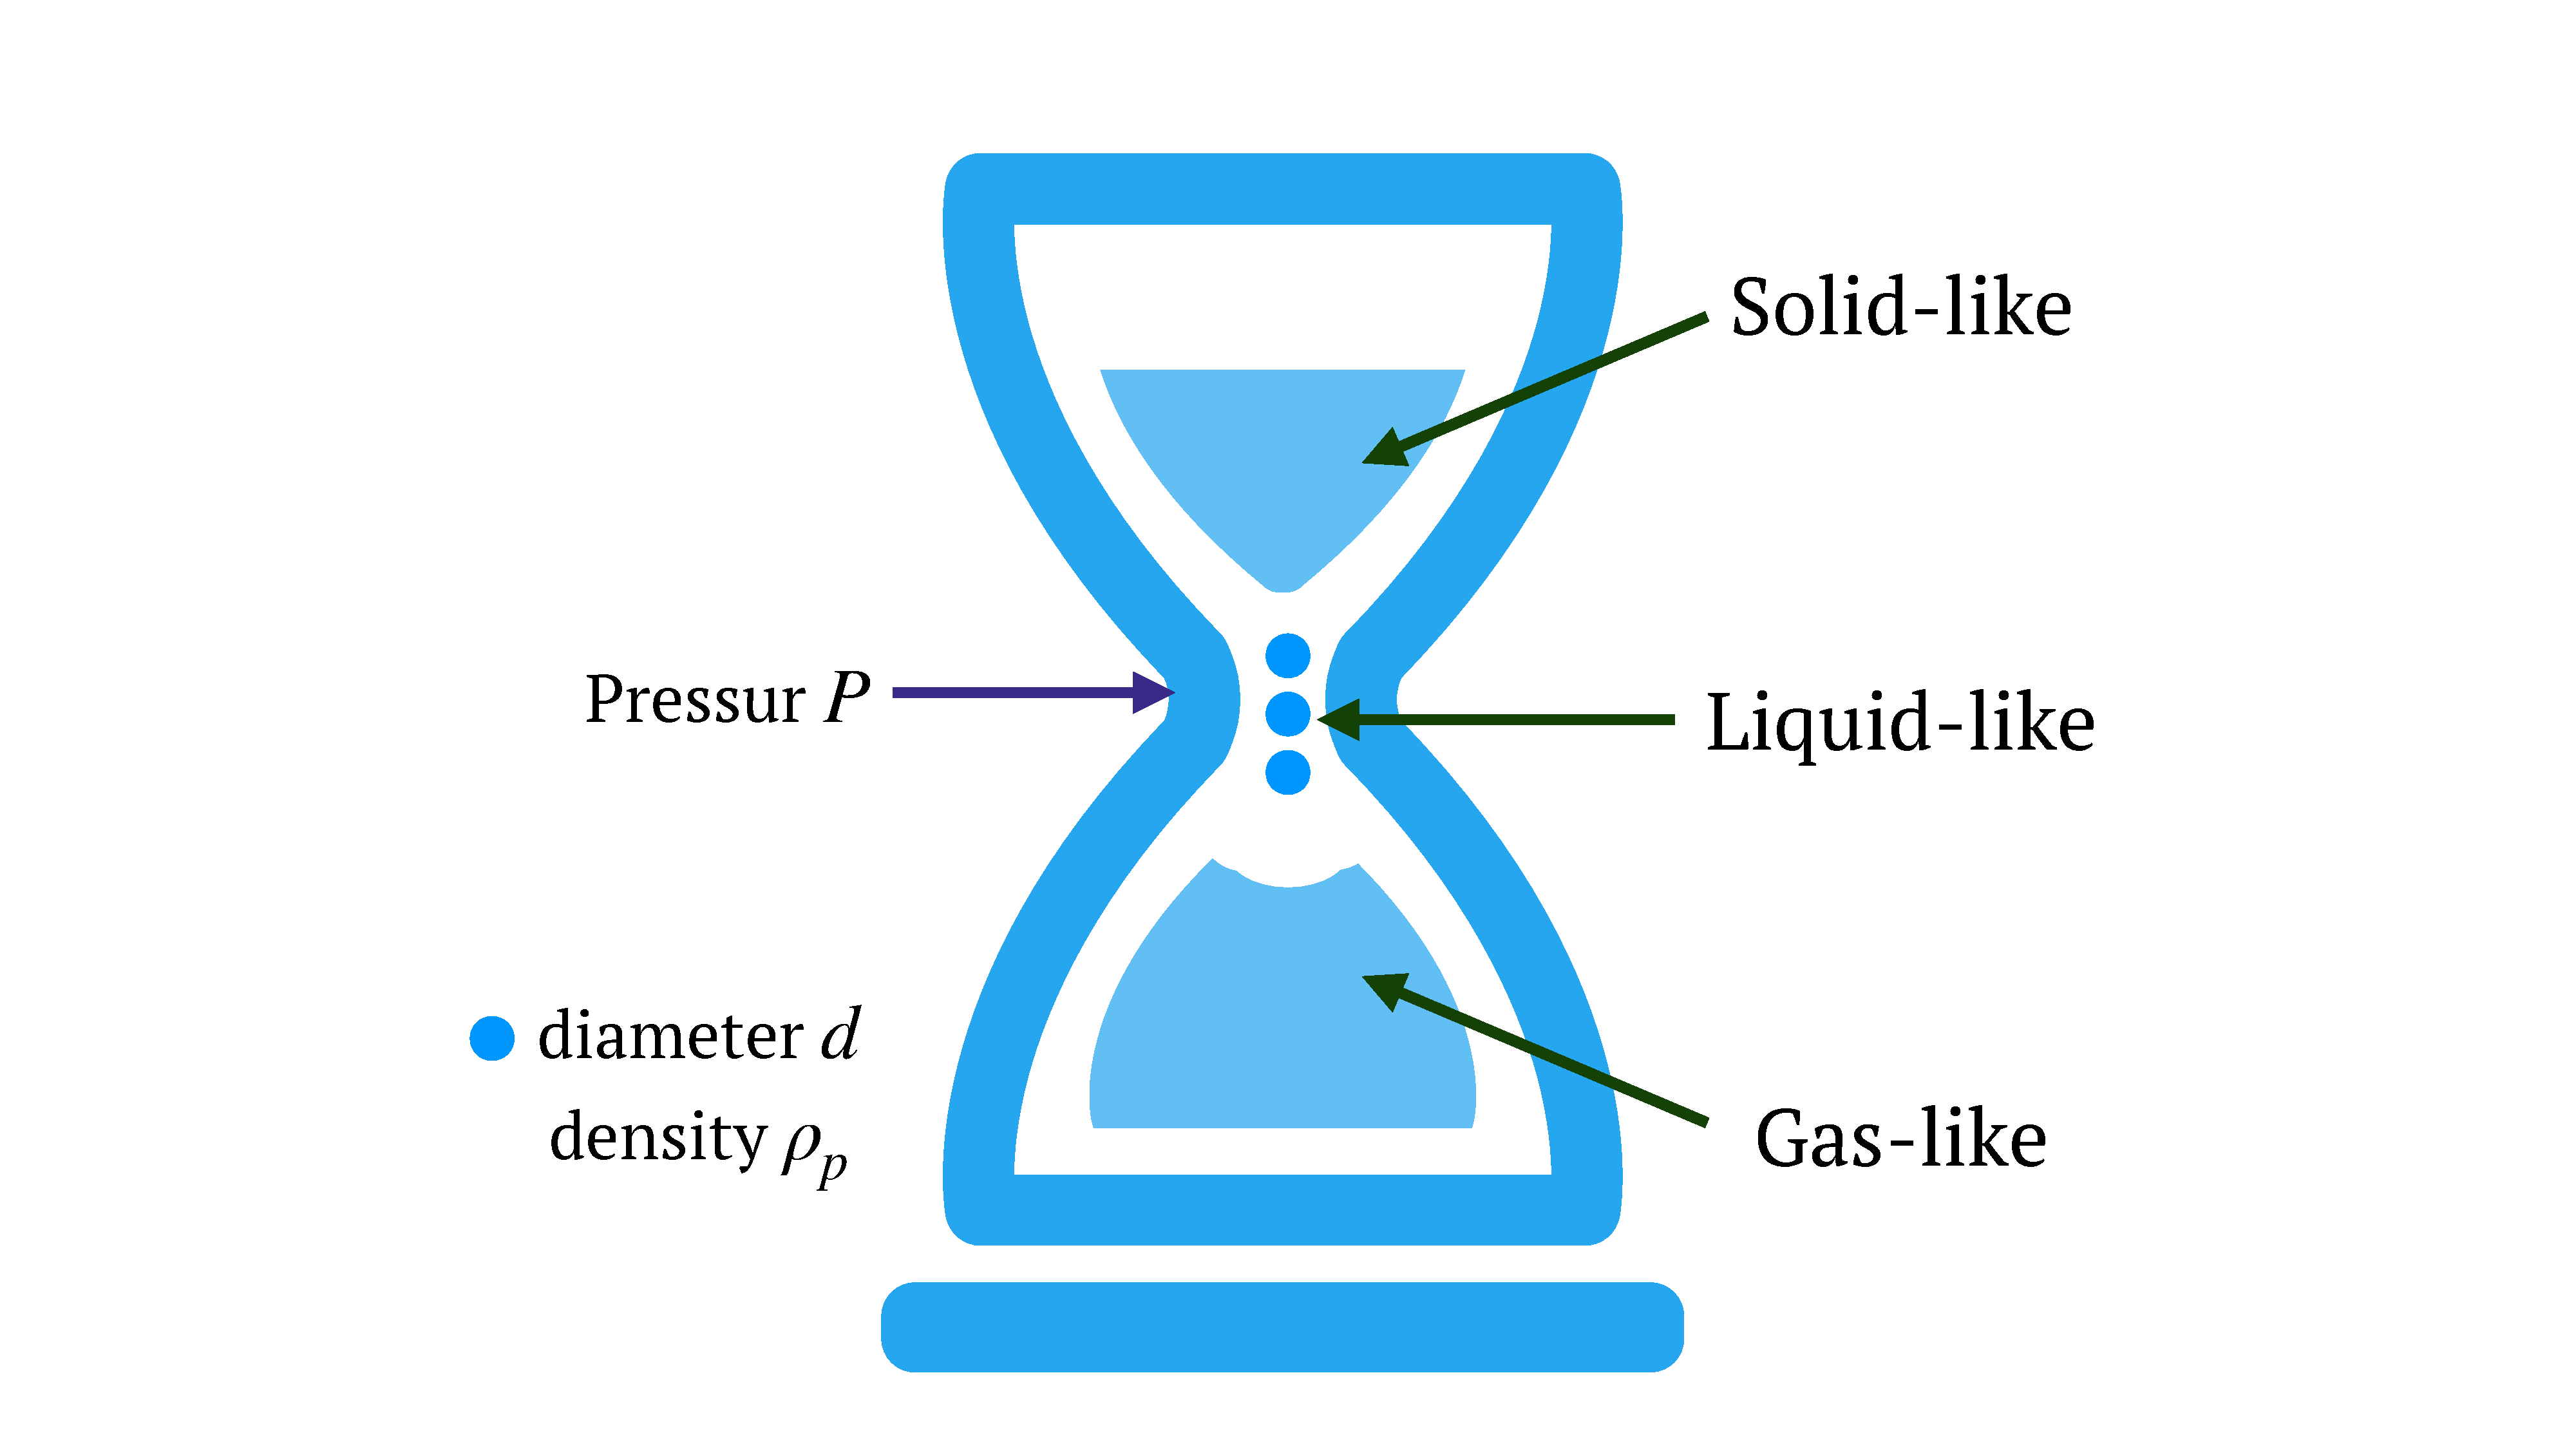
\includegraphics[scale=0.2]{figures/fig_hourglass.pdf}
    \end{center}
  \caption{Schematics of granular flow with an hourglass example.}
  \label{fig_hourglass}
\end{figure}
As we can see in Figure~\ref{fig_hourglass}, three different states can co-exist in granular materials. 
When we look at the top part of the hourglass, filled with sand, it typically seems not to move and resembles a solid. 
As we move our sight toward the middle nozzle of the hourglass, we can observe the sands passing through the nozzle, flowing like a liquid.
Meanwhile, the sand landing on the bottom part of the hourglass is forming a cone shape. When we look very closely at the top of the cone, we can see that the sand is falling and colliding, i.e., it behaves like a gas.
\par
In general, these three regimes can be categorized by the inertial number $I$. The solid-like status appears when $I$ is small. As the number $I$ increases, the flow deformation occurs rapidly, as we see in the middle of the hourglass. Naturally, the collisional flow can be observed for a large $I$ number. 
\par
By applying this $\mu(I)$ rheology, Srivastava~\cite{srivastava_viscometric_2021} devleoped a callibration to obtain the coefficients $\eta_i$ and $\kappa_i$.
For the first-order strain rate viscosity term, equation (\ref{eq_mu1_main}), we have 
\begin{equation}
  \mu_1(I) = \mu_1^0 + A_1{ I}^{ \alpha_1} =  \frac{(\eta_1 \dot{\gamma} + \kappa_1)}{P},\
\label{eq_muI1}
\end{equation}
where $\mu_1^0, A_1,$ and $\alpha_1$ are fitting parameters, depending on matrials. 
By substituting the inertial number $I$, equation (\ref{eq_inertialI}), into equation (\ref{eq_muI1}), we get
\begin{equation}
     \mu_1^0 + A_1 {\left(  \frac{\dot{\gamma} a }{\sqrt{P/\rho}}\right) }^{ \alpha_1} =  \frac{(\eta_1 \dot{\gamma} + \kappa_1)}{P}.
\end{equation}
We then find $\mu_1 (\dot{\gamma}, P)$ and $\kappa_1(p)$ as
\begin{equation}
    \mu_1  (\dot{\gamma}, P)= 
    \biggl( A_1 {\left(   d  \sqrt{\rho} \right) }^{ \alpha_1}\biggr) 
     \dot{\gamma}^{\alpha-1} P^{1-\alpha/2}
\label{eq_eta1}
\end{equation}
\begin{equation}
    \kappa_1(P) = \mu_1^0 P
\label{eq_kappa1}
\end{equation}
\par
Similarly, we can find the coefficients for the quadratic in ${\bm D}$ terms, having the $\mu(I)$ relationship as follows:
\begin{equation}
    \mu_2(I) = \mu_2^0 + A_2{ I^2}^{ \alpha_1} =  \frac{(\eta_2 \dot{\gamma}^2 + \kappa_2)}{P},\
\label{eq_muI2}
\end{equation}
Then, we obtain $\mu_2 (\dot{\gamma}, P)$ and $\kappa_2(P)$
\begin{equation}
    \mu_2  (\dot{\gamma}, P)= 
    \biggl( A_2 {\left(   d  \sqrt{\rho} \right) }^{ 2\alpha_2}\biggr) 
     {\dot{\gamma}}^{2(\alpha_2-1)} P^{1-\alpha_2}
\label{eq_eta2}
\end{equation}
\begin{equation}
    \kappa_2(P) = \mu_2^0 P
\label{eq_kappa2}
\end{equation}

%--------------------------------------------------
We can obtain the flow fitting parameters from particle-based simulations, such as the discrete element method (DEM). The following numbers are introduced in, Jop 2006 \cite{jop_constitutive_2006}; Srivastava 2021 \cite{srivastava_viscometric_2021}:
    \[
    0.09 \leq \mu_1^0 \leq 0.33, 
    \ \ \ \ \ \ \ 
    0.37 \leq \alpha_1 \leq 0.7
    \]
        \[
    0.01 \leq \mu_2^0 \leq 0.1, 
    \ \ \ \ \ \ \ 
    0.28 \leq \alpha_2 \leq 0.44.
    \]
            \[
    \ \ \ \ \ \ \ 
    0.75 \leq \alpha_3 \leq 0.85.
    \]
     One can find the corresponding $A_i$ values in Srivastava 2021 \cite{srivastava_viscometric_2021}.
\subsection{Computation of pressure-dependent apparent viscosity}
For granular rheology, it is typical to see compressible flow. It is, thus, essential to take pressure into account to evaluate viscosity.
Here, we consider the pressure as a combination of background flow pressure, $P_0$, that is linear in the vertical direction, and perturbation, $P'$ such that
\[
P = P_0(y) + P'(x,y,z).\]
Note that we can have the perturbations under gravity. Without gravitational force, we may simply input the constant pressure, $P_0$, and keep it over time.
\par
In case gravity is involved, we consider the density term, in order to approximate the perturbation, as 
\[
\rho  = \rho_0  + \rho'(x,y,z), 
\]
where $\rho_0$ is constant and $\rho'$ is spacial-dependant density perturbation of the flow. 
Here, we assume that 
\begin{equation}
    \nabla P_0  = \frac{d P_0}{d y} \approx \rho_0  g.  
\label{eq_p0_rho0}
\end{equation}
This recovers our momentum equation. As we would like to construct a background pressure that stays over time for our granular rheology, we may use this hidden assumption.
By taking integral both sides of Equation (\ref{eq_p0_rho0}), we obtain
\begin{equation}
    P_0 \approx p_{bg} + \nabla P_0 y.
\end{equation}
We would like to use this form since we already have the $p_{bg}$ term computed in the AMReX-incflo code.
%
When we have a periodic boundary in the gravity direction, we might need to prescribe a pressure gradient to have an additional pressure effect. 
\par
The main challenge we faced to implement the pressure-dependent viscosity was connecting the pressure in addition to the strain rate into the rheology code. To have physical consistency, we need to solve for a compressible flow model. We thus leave the pressure-dependent granular flow as a future work.
% {\color{blue} Are we keeping this the whole time? Is there any pressure change over time? Does a volume fraction come into play?}

% a little more details
\subsection{Viscosity regularization}
When we evaluate the viscosities, equations (\ref{eq_mu1_main}) and (\ref{eq_mu2_main}), we may encounter a (nearly) singularity as $\dot{\gamma}$ approaches zero.
As AMReX-incflo has the Papanastasiou regularization method implemented, we simply apply the same method for the new granular flow viscosity computations.
\par
By introducing a small parameter, denoted as $\varepsilon$, we can regularize the singularity of $\dot{\gamma}$ as following,
\[
  \frac{1}{\dot{\gamma}} \rightarrow \frac{1-e^{-\dot{\gamma} / \varepsilon}}{\dot{\gamma}}  
\]
for $\dot{\gamma}/\varepsilon \gg 1$. Otherwise, we simply use $1/\varepsilon$. 
The detailed mathematics and analysis can be found in Sverdrup 2018~\cite{sverdrup_highly_2018}.
\section{Suspension rheology}
This section summarizes the rheological model of suspensions in a Newtonian fluid. Solid particles suspended in a Newtonian fluid can exhibit highly non-Newtonian behaviors.  
\par
We use the constitutive equation proposed by Reiner \cite{reiner_mathematical_1945} and Rivlin \cite{rivlin_stress-deformation_1955},  
\begin{equation}
  \bar{\bar{\sigma}} = -P \bar{\bar{I}}
  + 2 \nu_1 {\bm{D}} + 2 \nu_2 {\bm{D}}^2.
\end{equation}
According to Tanner's review \cite{tanner_review_2018}, the coefficients $\nu_1$ can be constant since the rate of change with $\dot{\gamma}$ is negligible, and $\nu_2 = \beta / \dot{\gamma}$ for a suspension of solid particles in a Newtonian fluid, where a factor $\beta$ is related to the strain rate $\dot{\gamma}$. Dai et, al \cite{dai_viscometric_2013} shows the $\beta = -4.4 \phi^3 \nu_1$ in shear flows, where $\phi$ is a volume fraction. 
\par
For numerical validations, we follow the experiments presented in Couturier $\textit{et, al}$~\cite{couturier_suspensions_2011}.
\begin{itemize}
  \item We want to observe the relationship between $\alpha_i(\phi) = N_i / |\sigma_{xy}|$, where $i = 1,2$.
\end{itemize}

\section{Velocity computation}
Once we decide on a non-Newtonian model, in geometry, we solve flow velocity and pressure by solving the following Navier-Stokes equation,
\begin{equation}
  \nabla \cdot \vec{u} = 0 
  \label{eq_div_free} 
\end{equation}
\begin{equation}
     \frac{\partial \vec{u}}{\partial t} + \vec{u}\cdot \nabla \vec{u}
= \frac{1}{\rho}
\left(
- \nabla P 
    + \nabla \cdot   \bm{\tau} 
    +  \rho  \vec{g} 
    \right),
  \label{eq_NS_ch4}
  \end{equation}
where we find $\tau$ using equation (\ref{eq_2ndOrder_tau}) for a granular flow. 
Note that there are three integrations available in AMReX-incflo: 1) explicit Euler, 2) Crank-Nicolson, and 3) implicit Euler methods. 
Due to the non-linearity of the viscous term, $\bm{\tau}$, we began with the explicit Euler method during the internship. 
Focusing on the time integration, We first write the momentum equation in a discretized form, 
\begin{align}
    \vec{u}^*
= 
 \vec{u}^n + 
{\Delta t} 
\biggl(
-\vec{u}^n \cdot \nabla \vec{u}^n 
+\frac{1}{\rho}
\left(
- \nabla P^n 
    + \nabla \cdot   \bm{\tau}^n 
    +  \rho  \vec{g} 
    \right)
    \biggr),
  \end{align}
where the superscription $n$ represents the current time (known) value; for example, the current time (known) velocity is $\vec{u}^n = \vec{u}(\vec{x}, t_n)$. The new velocity value $\vec{u}^*$ is an updated velocity to the next time, i.e., $\vec{u}^* (\vec{x}, t_{n+1})$. However, it does not necessarily satisfy the continuity equation (\ref{eq_div_free}). Thus, we should project the intermediate velocity $\vec{u}^*$ onto the divergence-free space. 
\par
For the projection step, we express $\vec{u}^{*}$ as, according to the Helmholtz-Hodge-Decomposition~\cite{chorin_mathematical_1993}, 
\begin{equation}
  \vec{u}^* = \vec{u}^{n+1} + \nabla \phi,
  \label{eq_ustar}
\end{equation}
where $\vec{u}^{n+1}$ is the new velocity at time $t_n + \Delta t$ that satisfies the divergence-free condition and $\phi$ is a scalar function.
To take advantage of the nature of $\vec{u}^{n+1}$, we find the divergence of the equation (\ref{eq_ustar}), leading to the Poisson equation for $\phi$,
\[
  \nabla^2 \phi = \nabla \vec{u}^*.  
\]
After we solve for $\phi$, applying given boundary conditions, we find the updated velocity, projecting the velocity $\vec{u}^*$ onto the divergence-free space to get the new time-level solutions.
\[
  \vec{u}^{n+1} = \vec{u}^* - \nabla \phi.
\]

In this thesis, we focus on the time integration. 
Since an explicit scheme tends to show lower-order convergence and more stability issues, having an implicit method performing a higher-order convergence would be beneficial.  
\subsection{Explicit Runge-Kutta 2 (RK2)}
As an easier step, we first try out the second-order Runge-Kutta method. We already introduced this scheme for solving the advection-diffusion equation in Chapter \ref{sec:AD_times}. We recall here, 
\begin{align}
	\vec{u}_{j}^{temp} = \vec{u}^{n} + \frac{\Delta t}{2} {\bm F} \left( \vec{u}^{n} \right)
	\label{eq_RK2_s1} \\ 
	\vec{u}^{n+1} = \vec{u}^{n} + \Delta t {\bm F} \left( \vec{u}^{temp} \right),
	\label{eq_RK2_s2}
\end{align}
where 
\[
  {\bm F} = 
    -\vec{u}^n \cdot \nabla \vec{u}^n 
    +\frac{1}{\rho}
    \left(
    - \nabla P^n 
        + \nabla \cdot   \bm{\tau}^n 
        +  \rho  \vec{g} 
        \right).
\]


\subsection{Predictor-Corrector method}
To enlarge the numerical stability region, we implement a semi-implicit method. To do so, we first re-write the momentum equation by splitting the deviatoric stress tensor, ${\bm \tau}$, into two parts, 
\[
 {\bm \tau}= {\bm \tau_1} + {\bm \tau_2},
\] 
where ${\bm \tau_1}$ and ${\bm \tau_2}$ are, respectively, the linear and quadratic relationship with ${\bm D}$, i.e., 
\[
  {\boldsymbol \tau_1} \propto \boldsymbol{D}
  \ \ \ \ \ \text{and}
   \ \ \ \ \ 
{\boldsymbol \tau_2} \propto {\boldsymbol D^2}.
\]
We denote the advection term, $\vec{u} \cdot \nabla \vec{u}$ as ${\bm A}$. 
\\
$<${\bf Predictor}$>$
\\
First, consider the non-linear stress tensor, ${\bm \tau_2}$ as a force term, and solve for the first predictor values, that are $\vec{u}^*$ and $\vec{u}^*$:
\[
\frac{{\color{blue}\vec{u}^*} - \vec{u}^n}{\Delta t} 
+  {\bm A}^{n+1/2} 
= \frac{1}{\rho}  \biggl(
\frac{\nabla \cdot {\color{blue}{\bm \tau}_1^*} + \nabla \cdot{\bm \tau}_1^n}{2} 
+ \nabla \cdot {\bm \tau}_2^n 
- \nabla p^n
+{\bm g}
\biggr)
\]
We solve for blue terms - 
\[
{\color{blue}\vec{u}^*} -
\frac{\Delta t}{\rho} 
\left( 
\frac{\nabla \cdot {\color{blue}{\bm \tau}_1^*}}{2}
\right)
=
\vec{u}^n
- {\bm A}^{n+1/2} \Delta t
+ \frac{\Delta t}{\rho} \biggl(
\frac{ \nabla \cdot{\bm \tau}_1^n}{2} 
+ \nabla \cdot {\bm \tau}_2^n 
- \nabla p^n
+{\bm g}
\biggr)
\]
\\
$<${\bf Corrector}$>$
\\
Once we obtain the predictor (star) velocity, we use it to compute the second order stress tensor, ${\bm \tau}_2^*$.
\[
\frac{{\color{red}\vec{u}^{n+1}} - \vec{u}^n}{\Delta t} 
+  {\bm A}^{n+1/2} 
=  \frac{1}{\rho}  \biggl(
\frac{\nabla \cdot {\color{red}{\bm \tau}_1^{n+1}} + \nabla \cdot{\bm \tau}_1^n}{2} 
+ \frac{\nabla \cdot {\bm \tau}_2^{n} + \nabla \cdot {\color{blue}{\bm \tau}_2^*}}{2} 
- \nabla p^n
\biggr)
\]

Now, we need to solve for red - next time step values:
\[
{\color{red}\vec{u}^{n+1}} 
-\frac{1}{\rho} 
\left(
\frac{\nabla \cdot {\color{red}{\bm \tau}_1^{n+1}}}{2}
\right)
=
\vec{u}^n 
 -{\bm A}^{n+1/2} \Delta t
 +\frac{\Delta t}{\rho}  \biggl(
\frac{ \nabla \cdot{\bm \tau}_1^n}{2} 
+ \frac{\nabla \cdot {\bm \tau}_2^{n} + \nabla \cdot {\color{blue}{\bm \tau}_2^*}}{2} 
- \nabla p^n
\biggr)
\]
Note that ${\bm \tau}_i^* = {\bm \tau}(\vec{u}^*, \eta_i)$.






\section{Numerical results}
\begin{itemize}
  \item We follow the experiment setup found in \cite{couturier_suspensions_2011}
  \item We want to present the N1 and N2 values with various volume fractions: from 0.1 to 0.5.
  \item the geometry of a tilted trough with rigid spheres in a Newtonian fluid. 
\end{itemize}

\section{Discussion and future work}
We may add the time-dependent flow presented in the last term in the following equation
\begin{equation}
  \bm{\tau} =  \mu_1 {\bm D} 
    + \mu_2  \left[ {\bm D}^2  - \frac{\text{tr}\left({\bm D}^2\right)}{3}{\bm I} \right]
   + \kappa_1 \frac{{\bm D}}{|{\bm D}|} 
    + \kappa_2  \left[ \frac{{\bm D}^2}{|{\bm D}|^2}  
    - \frac{\text{tr}\left({\bm D}^2\right)}{3|{\bm D}|^2}{\bm I} \right]
    + \mu_3  \left[ {\bm D}{\bm W} - {\bm W}{\bm D} \right]
  \end{equation}
  For the last coefficient in equation (\ref{eq_2ndOrder_tau}), we follow the power law, 
\begin{equation}
    \mu_3(I) = -A_3 \left( I^2 \right)^{\alpha_3} = \frac{\eta_3 \dot{\gamma}^2}{p}.
\label{eq_muI3}
\end{equation}
Specifically, we can find the coefficients of each shear rate term in Equation (\ref{eq_2ndOrder_tau}) as
\begin{equation}
     \eta_3 (\dot{\gamma}, p) = 
    -p A_3 
        \left( \frac{\dot{\gamma} a }{\sqrt{p/\rho}}  \right)^{2\alpha_3} 
        \frac{1}{\dot{\gamma}^2},
\label{eq_gr_eta_3}
\end{equation}
\par
We propose to extend this work by incorporating elastic effects through the implementation of elastoviscoplastic (EVP) models in this numerical framework. The robustness of the numerical implementation will be extensively tested in various flow scenarios (such as Poiseuille and Couette flows) for a range of Weissenberg and Bingham numbers.  Another potential avenue for development will involve implementing immersed boundary methods (IBM) to model a suspension of solid particles in such complex fluids, which is an important application area that has received significant research interest lately. 
\par
Add surface tension effect inAMReX-incflo. 
\par 
As a personal research interest, I would like to study more about biofluids to contribute to a blood separation method. 